\section{Extended Ablation Study}
This section is new in the revision. All experiments use the protocol of Section~IV-G: raw data, all preprocessing inside training folds, identical splits and fixed hyper-parameters for every variant, paired differences with corrected 95\% CIs, and Holm-adjusted p-values. In total \nVariants{} configurations were evaluated. Code and all result tables are in the accompanying notebook (Section~17B) and repository.

\begin{table*}[!t]
\centering
\scriptsize
\caption{Component ablation under the controlled protocol (5$\times$10-fold repeated CV, 50 paired folds, fixed hyper-parameters, all preprocessing inside folds). $\Delta$AUC is paired against the full system; CIs use the Nadeau--Bengio correction.}
\label{tab:e1}
\setlength{\tabcolsep}{3pt}
\begin{adjustbox}{max width=\linewidth}
\begin{tabular}{lcccccccc}
\toprule
Variant & AUC [95\% CI] & Acc. & Sens. & Spec. & F1 & Brier & $\Delta$AUC [95\% CI] & $p_{\mathrm{Holm}}$ \\
\midrule
Full system (clinical + ECG-proxy, SMOTE, soft voting) & 0.902 [0.858, 0.945] & 0.823 & 0.773 & 0.867 & 0.799 & 0.127 & -- & -- \\
\midrule
$-$ ECG-proxy block (clinical only) & 0.906 [0.864, 0.947] & 0.826 & 0.789 & 0.858 & 0.805 & 0.126 & +0.004 [-0.009, +0.017] & 1.000 \\
$-$ clinical block (ECG-proxy only) & 0.813 [0.758, 0.867] & 0.769 & 0.708 & 0.820 & 0.737 & 0.175 & -0.089 [-0.132, -0.046] & 0.003 \\
\midrule
$-$ duplicated raw proxy columns & 0.902 [0.858, 0.946] & 0.827 & 0.771 & 0.874 & 0.801 & 0.126 & +0.000 [-0.004, +0.005] & 1.000 \\
$-$ polynomial terms & 0.902 [0.858, 0.945] & 0.828 & 0.777 & 0.872 & 0.804 & 0.127 & +0.000 [-0.004, +0.004] & 1.000 \\
$-$ interaction terms & 0.902 [0.858, 0.946] & 0.822 & 0.773 & 0.864 & 0.798 & 0.126 & +0.001 [-0.004, +0.005] & 1.000 \\
$-$ log transforms & 0.902 [0.858, 0.945] & 0.827 & 0.774 & 0.873 & 0.803 & 0.127 & -0.000 [-0.004, +0.004] & 1.000 \\
$-$ ratio features & 0.901 [0.857, 0.945] & 0.825 & 0.781 & 0.863 & 0.803 & 0.127 & -0.001 [-0.006, +0.005] & 1.000 \\
$-$ threshold flags & 0.900 [0.858, 0.943] & 0.823 & 0.768 & 0.869 & 0.797 & 0.127 & -0.001 [-0.009, +0.006] & 1.000 \\
$-$ HR-reserve features & 0.901 [0.857, 0.944] & 0.826 & 0.780 & 0.866 & 0.803 & 0.127 & -0.001 [-0.006, +0.004] & 1.000 \\
$-$ ischaemia composite & 0.902 [0.858, 0.945] & 0.826 & 0.774 & 0.869 & 0.801 & 0.127 & +0.000 [-0.005, +0.006] & 1.000 \\
downslope coding fixed (slope==3) & 0.902 [0.858, 0.946] & 0.823 & 0.776 & 0.864 & 0.800 & 0.127 & +0.000 [-0.003, +0.004] & 1.000 \\
\midrule
$-$ SMOTE (no resampling) & 0.900 [0.855, 0.945] & 0.834 & 0.763 & 0.895 & 0.806 & 0.128 & -0.002 [-0.009, +0.006] & 1.000 \\
\midrule
$-$ soft voting $\rightarrow$ XGBoost only & 0.895 [0.850, 0.939] & 0.821 & 0.771 & 0.863 & 0.796 & 0.132 & -0.007 [-0.020, +0.006] & 1.000 \\
$-$ soft voting $\rightarrow$ SVM only & 0.905 [0.862, 0.949] & 0.840 & 0.815 & 0.861 & 0.823 & 0.121 & +0.004 [-0.015, +0.023] & 1.000 \\
$-$ soft voting $\rightarrow$ GBM only & 0.884 [0.840, 0.927] & 0.801 & 0.757 & 0.839 & 0.775 & 0.139 & -0.018 [-0.034, -0.002] & 0.558 \\
$-$ soft voting $\rightarrow$ RF only & 0.880 [0.831, 0.929] & 0.817 & 0.771 & 0.856 & 0.793 & 0.139 & -0.022 [-0.041, -0.002] & 0.510 \\
$-$ soft voting $\rightarrow$ logistic regression & 0.898 [0.853, 0.942] & 0.838 & 0.823 & 0.851 & 0.824 & 0.125 & -0.004 [-0.025, +0.017] & 1.000 \\
soft $\rightarrow$ hard (majority) voting & 0.869 [0.818, 0.920] & 0.812 & 0.796 & 0.825 & 0.793 & 0.147 & -0.032 [-0.053, -0.011] & 0.067 \\
soft voting $\rightarrow$ stacking (LR meta-learner) & 0.902 [0.857, 0.946] & 0.824 & 0.783 & 0.859 & 0.802 & 0.124 & -0.000 [-0.005, +0.005] & 1.000 \\
\midrule
Clinical only, no SMOTE, logistic regression & 0.904 [0.862, 0.946] & 0.835 & 0.794 & 0.871 & 0.814 & 0.123 & +0.003 [-0.017, +0.022] & 1.000 \\
\bottomrule
\end{tabular}
\end{adjustbox}
\end{table*}


\subsection{Component Ablation (RQ1, RQ2)}
Table~\ref{tab:e1} and Fig.~\ref{fig:a1} remove one component at a time. Under leak-free repeated CV the full system reaches AUC \fullAUC{} \fullAUCci{}, accuracy \fullAcc{}, sensitivity \fullSens{} and specificity \fullSpec{}. These figures are clearly lower than the v4 hold-out values (0.9535, 0.8852, 0.9286).

\textbf{ECG-proxy block.} Removing the entire proxy block (clinical only) changes AUC by \dClinAUC{} and accuracy by \dClinAcc{}~pp; the clinical-only system is numerically \emph{slightly better}. No individual feature group (polynomial, interaction, log, ratio, threshold, HR-reserve, ischaemia composite or the duplicated raw columns) changes AUC by more than \engMaxAbs{}. Correcting the ``downslope'' coding has no measurable effect. On its own, the proxy block is informative but clearly weaker than the clinical variables (proxy-only $\Delta$AUC \dProxyOnlyAUC{}, $p_{\text{Holm}}=\pProxyOnly{}$).

\textbf{SMOTE.} Removing SMOTE changes AUC by \dNoSmoteAUC{} and accuracy by \dNoSmoteAcc{}~pp. The v4 claim that SMOTE removal causes the largest drop (``$\approx$3.3\%'') is not reproduced. Without resampling, specificity rises (\noSmoteSpec{}) and sensitivity falls slightly (\noSmoteSens{}), as expected when the training prior is no longer artificially balanced.

\textbf{Ensemble.} Random forest alone ($\Delta$AUC \dRfOnlyAUC{}) and GBM alone (\dGbmOnlyAUC{}) have lower AUC than soft voting. Their uncorrected CIs exclude zero, but neither difference is significant after Holm correction ($p_{\text{Holm}}=\pRfOnly{}$ and \pGbmOnly{}). Soft voting does not outperform an RBF-SVM alone (\dSvmOnlyAUC{}) or plain logistic regression (\dLRAUC{}). Hard voting has the lowest AUC (\dHardAUC{}, $p_{\text{Holm}}=\pHard{}$), partly by construction: a four-member vote yields only five distinct scores, which limits ranking-based metrics. Stacking matches soft voting (\dStackAUC{}). A clinical-only logistic regression without any resampling reaches AUC \clinLRAUCval{} ($\Delta$ \dClinLRAUC{}), statistically indistinguishable from the full system.

\begin{figure}[!t]
\centering
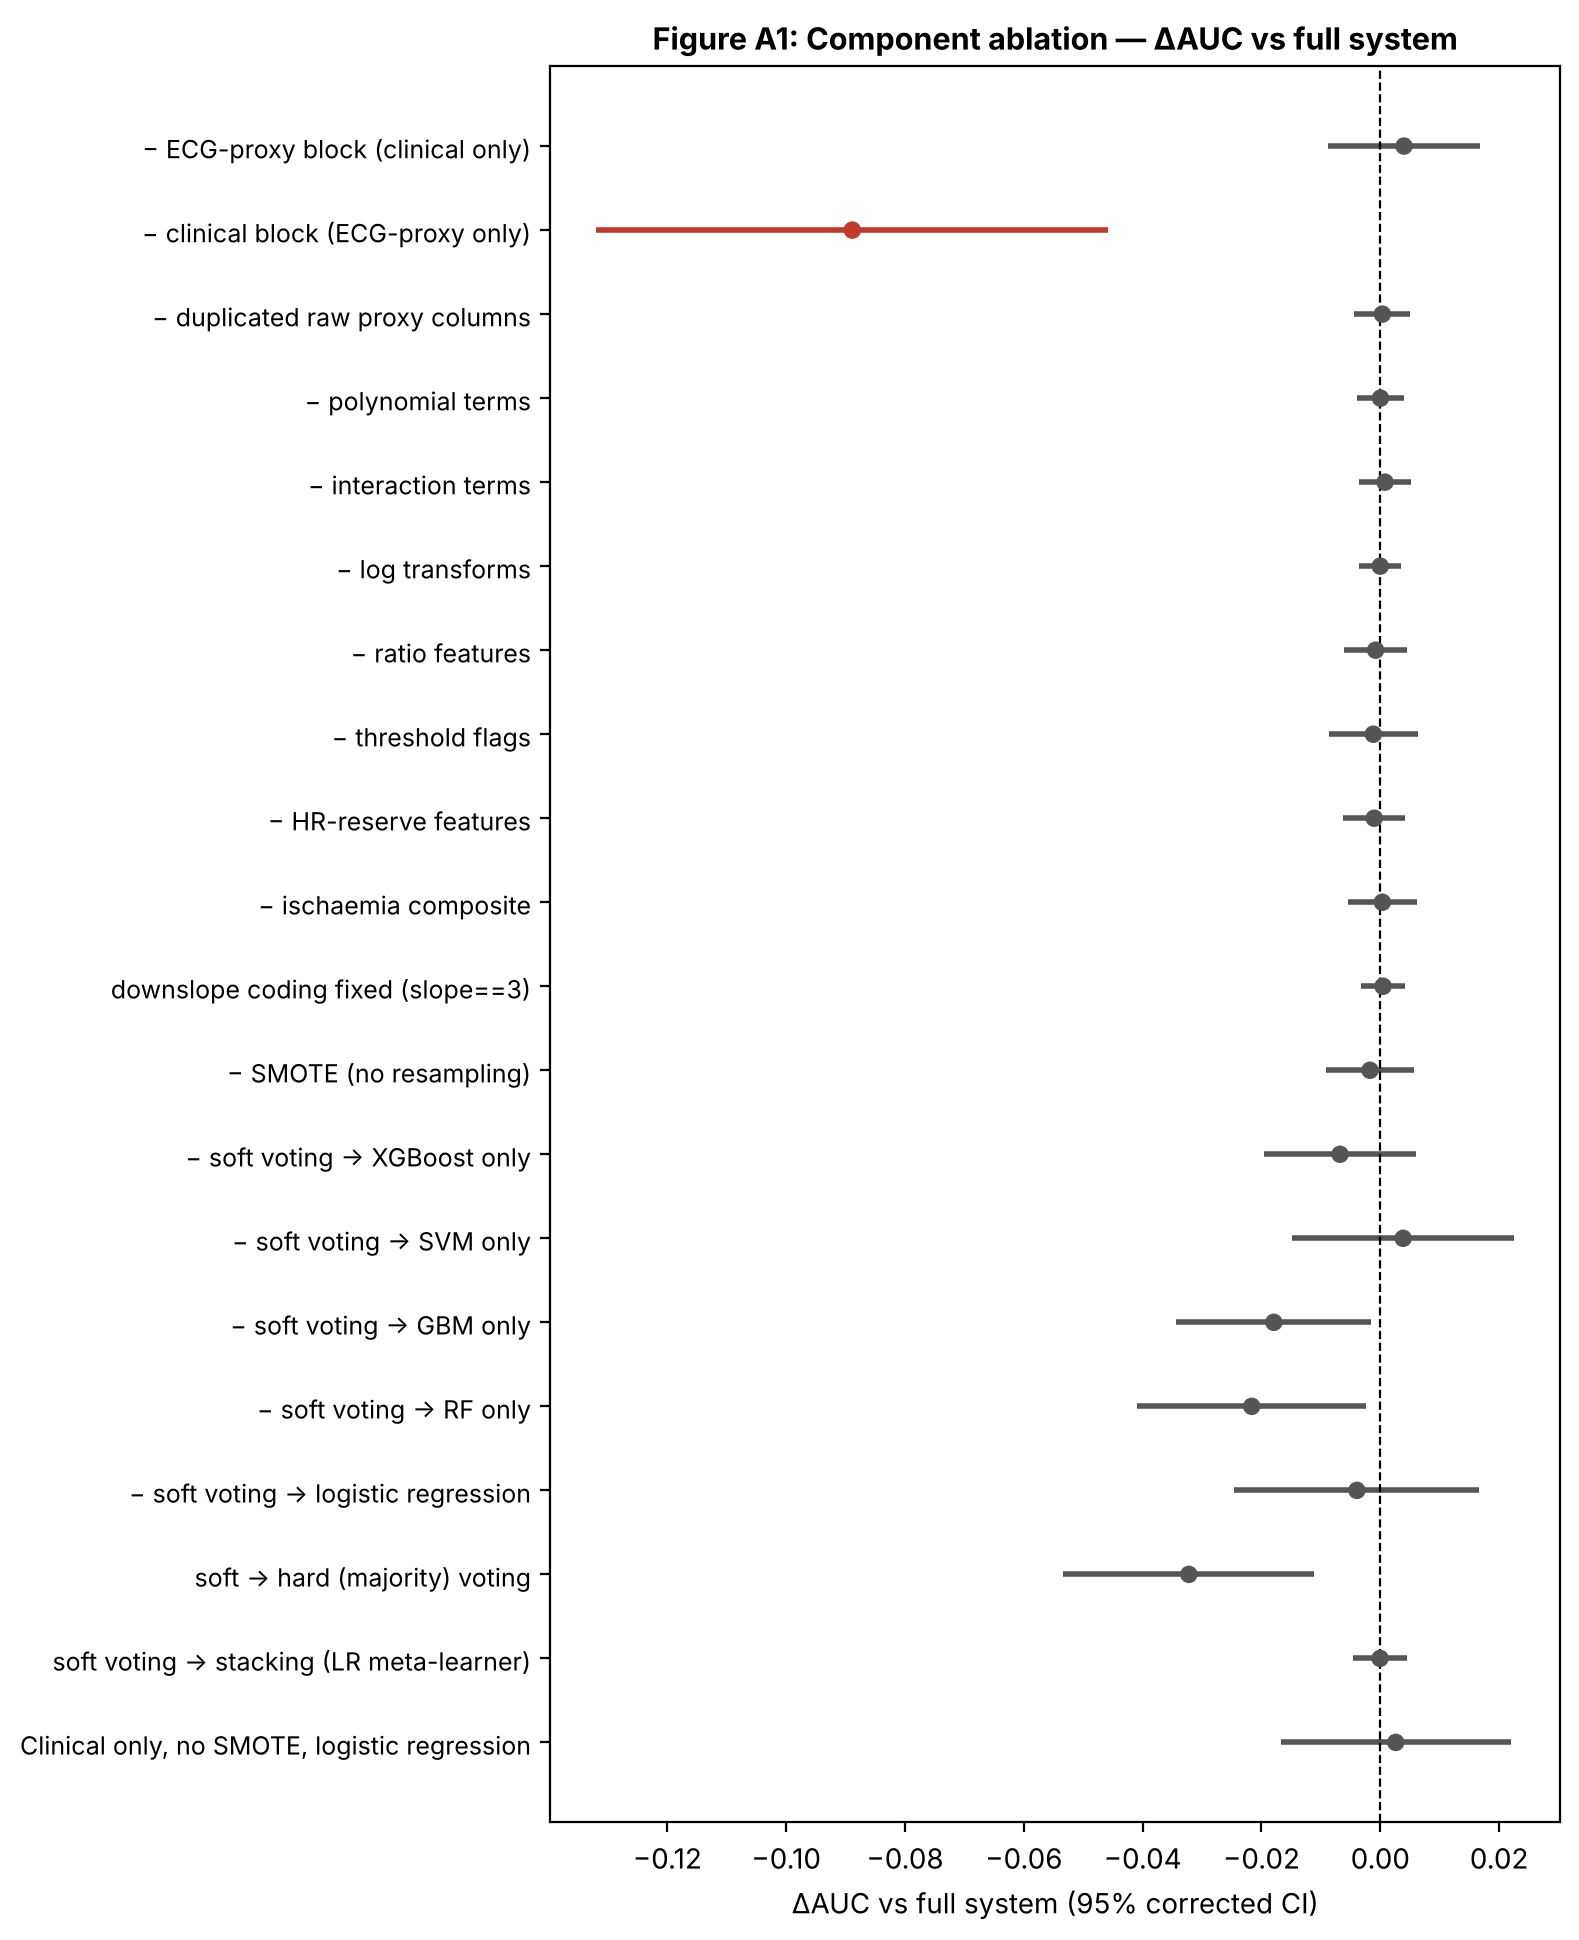
\includegraphics[width=\linewidth]{figA1_component_ablation.png}
\caption{Component ablation: paired $\Delta$AUC versus the full system with 95\% corrected CIs (grey = not significant after Holm correction).}
\label{fig:a1}
\end{figure}

\subsection{Control Experiments}
If the proxy block carried information beyond the clinical variables, it should outperform equally sized blocks of irrelevant features. Table~\ref{tab:e2} shows that it does not. Clinical + 18 engineered \emph{non-ECG} features (cholesterol, blood pressure and age transforms) reach AUC \nonecgAUC{}, clinical + 18 pure \emph{Gaussian-noise} columns \noiseAUC{}, and clinical + a \emph{row-shuffled} proxy block \shuffledAUC{}, all within the CI of the full system. This is expected: the proxy features are deterministic functions of variables the classifiers already see, and tree ensembles and RBF-SVMs can represent such products and ratios themselves. A label-permutation test confirms that the full system learns real signal (observed AUC \permObs{} versus \permNull{}$\pm$\permNullSd{} under \permN{} permutations, $p=\permP{}$, the smallest value attainable with \permN{} permutations).

\begin{table*}[!t]
\centering
\scriptsize
\caption{Control experiments: is the ECG-proxy block better than other added features?}
\label{tab:e2}
\setlength{\tabcolsep}{3pt}
\begin{adjustbox}{max width=\linewidth}
\begin{tabular}{lcccc}
\toprule
Feature set (soft voting, SMOTE) & AUC [95\% CI] & Acc. & $\Delta$AUC vs full & $p_{\mathrm{Holm}}$ \\
\midrule
Full system (clinical + ECG-proxy, SMOTE, soft voting) & 0.902 [0.858, 0.945] & 0.823 & -- & -- \\
Clinical only & 0.906 [0.864, 0.947] & 0.826 & +0.004 [-0.009, +0.017] & 1.000 \\
Clinical + 18 engineered non-ECG features & 0.903 [0.861, 0.946] & 0.822 & +0.002 [-0.016, +0.020] & 1.000 \\
Clinical + 18 Gaussian-noise features & 0.899 [0.855, 0.943] & 0.824 & -0.003 [-0.023, +0.018] & 1.000 \\
Clinical + row-shuffled ECG-proxy block & 0.897 [0.850, 0.944] & 0.826 & -0.004 [-0.020, +0.011] & 1.000 \\
Clinical + ECG-proxy + non-ECG features & 0.902 [0.859, 0.944] & 0.822 & +0.000 [-0.011, +0.012] & 1.000 \\
\bottomrule
\end{tabular}
\end{adjustbox}
\end{table*}


\subsection{Class-Imbalance Strategies}
Cleveland is only mildly imbalanced (54.1\%/45.9\%), and Table~\ref{tab:e3} shows that the choice of strategy hardly matters: no correction, class weighting, random oversampling, SMOTE after or before feature derivation, SMOTE-NC~\cite{chawla2002}, Borderline-SMOTE~\cite{han2005borderline} and ADASYN~\cite{he2008adasyn} all lie within $\pm$0.005 AUC of each other, with no significant differences. SMOTE does, however, create implausible patients: in the first training fold \smoteNonInt{} of the synthetic rows carry non-integer categorical codes (e.g.\ chest-pain type 2.6), and when SMOTE is applied after feature derivation \smoteInconsistent{} of synthetic rows have oldpeak$^2$ differing from the square of their oldpeak by more than 5\%. Because it brings no measurable benefit here, we recommend class weighting or no correction for this dataset, and SMOTE-NC on raw rows where oversampling is required. Table~\ref{tab:counts} gives the class counts per partition.

\begin{table*}[!t]
\centering
\scriptsize
\caption{Class-imbalance strategies (full feature set, soft voting; resampling inside training folds only). Calibration slope: ideal 1; $>$1 means under-confident probabilities.}
\label{tab:e3}
\setlength{\tabcolsep}{3pt}
\begin{adjustbox}{max width=\linewidth}
\begin{tabular}{lcccccc}
\toprule
Imbalance strategy & AUC & Sens. & Spec. & Brier & Cal.\ slope & $\Delta$AUC [95\% CI] \\
\midrule
SMOTE after features (paper) & 0.902 & 0.773 & 0.867 & 0.127 & 1.37 & -- \\
No correction & 0.900 & 0.763 & 0.895 & 0.128 & 1.41 & -0.002 [-0.009, +0.006] \\
Class weighting (no resampling) & 0.901 & 0.768 & 0.882 & 0.127 & 1.42 & -0.001 [-0.007, +0.005] \\
Random oversampling & 0.897 & 0.771 & 0.867 & 0.129 & 1.40 & -0.005 [-0.013, +0.003] \\
SMOTE on raw rows $\rightarrow$ derive proxy & 0.899 & 0.774 & 0.867 & 0.128 & 1.36 & -0.003 [-0.010, +0.005] \\
SMOTE-NC on raw rows $\rightarrow$ derive proxy & 0.900 & 0.771 & 0.872 & 0.128 & 1.37 & -0.002 [-0.009, +0.005] \\
Borderline-SMOTE & 0.900 & 0.789 & 0.851 & 0.129 & 1.39 & -0.001 [-0.010, +0.008] \\
ADASYN & 0.903 & 0.779 & 0.868 & 0.126 & 1.45 & +0.001 [-0.006, +0.008] \\
\bottomrule
\end{tabular}
\end{adjustbox}
\end{table*}

\begin{table}[!t]
\centering
\scriptsize
\caption{Class counts per partition (H = healthy, D = disease). SMOTE is fitted on training rows only.}
\label{tab:counts}
\setlength{\tabcolsep}{3pt}
\begin{adjustbox}{max width=\linewidth}
\begin{tabular}{lccc}
\toprule
Partition & Train (H/D) & After SMOTE & Test (H/D) \\
\midrule
D1/D3 Cleveland (80/20 hold-out) & 131/111 & 131/131 & 33/28 \\
D1/D3 Cleveland (one 10-fold CV fold) & 147/125 & 147/147 & 17/14 \\
\bottomrule
\end{tabular}
\end{adjustbox}
\end{table}


\subsection{Evaluation Protocol and Leakage}
Table~\ref{tab:e4} quantifies protocol choices. Fitting imputation and scaling on all 303 patients (as in v4) has negligible effect here (AUC \leakPreAUC{}), because only six values are missing and the scaler's statistics hardly change. Applying SMOTE \emph{before} cross-validation, however, inflates AUC to \leakSmoteAUC{}, because synthetic neighbours of test patients enter the training folds. Errors of this kind could contribute to some very high accuracies reported in the literature, although we cannot tell which published studies, if any, are affected. Fully nested tuning of XGBoost (AUC \nestedAUC{}) performs similarly to the fixed Section-15 parameters (\fixedXgbAUC{}) and better than library defaults (\defaultXgbAUC{}), so the fixed parameters introduce no detectable optimism.

\begin{table*}[!t]
\centering
\scriptsize
\caption{Leakage and tuning protocol (5$\times$10-fold CV). Leaky rows are shown only to quantify the bias.}
\label{tab:e4}
\setlength{\tabcolsep}{3pt}
\begin{adjustbox}{max width=\linewidth}
\begin{tabular}{lccc}
\toprule
Protocol & AUC [95\% CI] & Accuracy [95\% CI] & Sensitivity [95\% CI] \\
\midrule
Leak-free CV (reference) & 0.902 [0.858, 0.945] & 0.823 [0.766, 0.881] & 0.773 [0.686, 0.860] \\
Leaky (a): preprocessing fitted on all rows & 0.902 [0.859, 0.945] & 0.823 [0.765, 0.881] & 0.773 [0.685, 0.861] \\
Leaky (b): SMOTE before CV & 0.916 [0.877, 0.955] & 0.838 [0.793, 0.884] & 0.794 [0.718, 0.870] \\
XGBoost, fixed Section-15 params & 0.895 [0.850, 0.939] & 0.821 [0.764, 0.877] & 0.771 [0.684, 0.859] \\
XGBoost, nested tuning (inner 3-fold) & 0.900 [0.859, 0.942] & 0.822 [0.767, 0.877] & 0.780 [0.695, 0.865] \\
XGBoost, library defaults & 0.875 [0.831, 0.919] & 0.789 [0.732, 0.847] & 0.749 [0.664, 0.834] \\
\bottomrule
\end{tabular}
\end{adjustbox}
\end{table*}


\textbf{Hold-out sensitivity.} The v4 headline numbers come from one 80/20 split (seed 42). Repeating the identical leak-free pipeline on \hoN{} random 80/20 splits (Table~\ref{tab:holdout}, Fig.~\ref{fig:a3}) gives a mean fused accuracy of \hoFuAcc{}, while seed 42 gives \hoFuAccSeed{}, the \hoFuAccPct{}th percentile. For fused AUC, seed 42 lies at the \hoFuAUCPct{}th percentile. The fused$-$clinical accuracy difference averages \hoDAcc{} across splits, so a single favourable split can produce an apparent gain of several points by chance. Single 61-patient hold-out results on this dataset should therefore always be accompanied by repeated-split or repeated-CV estimates.

\begin{table*}[!t]
\centering
\scriptsize
\caption{Sensitivity of the 61-patient hold-out estimate to the random split (leak-free pipeline). ``Pct. is the percentile of the seed-42 split used in the v4 paper.}
\label{tab:holdout}
\setlength{\tabcolsep}{3pt}
\begin{adjustbox}{max width=\linewidth}
\begin{tabular}{lccc}
\toprule
Metric & Mean (2.5--97.5\%) over random 80/20 splits & Seed 42 & Pct. \\
\midrule
Fused accuracy & 0.833 (2.5--97.5\%: 0.754--0.918) & 0.902 & 95 \\
Clinical accuracy & 0.831 (2.5--97.5\%: 0.738--0.902) & 0.869 & 81 \\
Fused $-$ clinical accuracy & 0.002 (2.5--97.5\%: -0.049--0.049) & 0.033 & 90 \\
Fused AUC & 0.904 (2.5--97.5\%: 0.832--0.955) & 0.96 & 99 \\
Clinical AUC & 0.911 (2.5--97.5\%: 0.840--0.960) & 0.948 & 90 \\
Fused $-$ clinical AUC & -0.007 (2.5--97.5\%: -0.034--0.017) & 0.012 & 94 \\
\bottomrule
\end{tabular}
\end{adjustbox}
\end{table*}


\begin{figure}[!t]
\centering
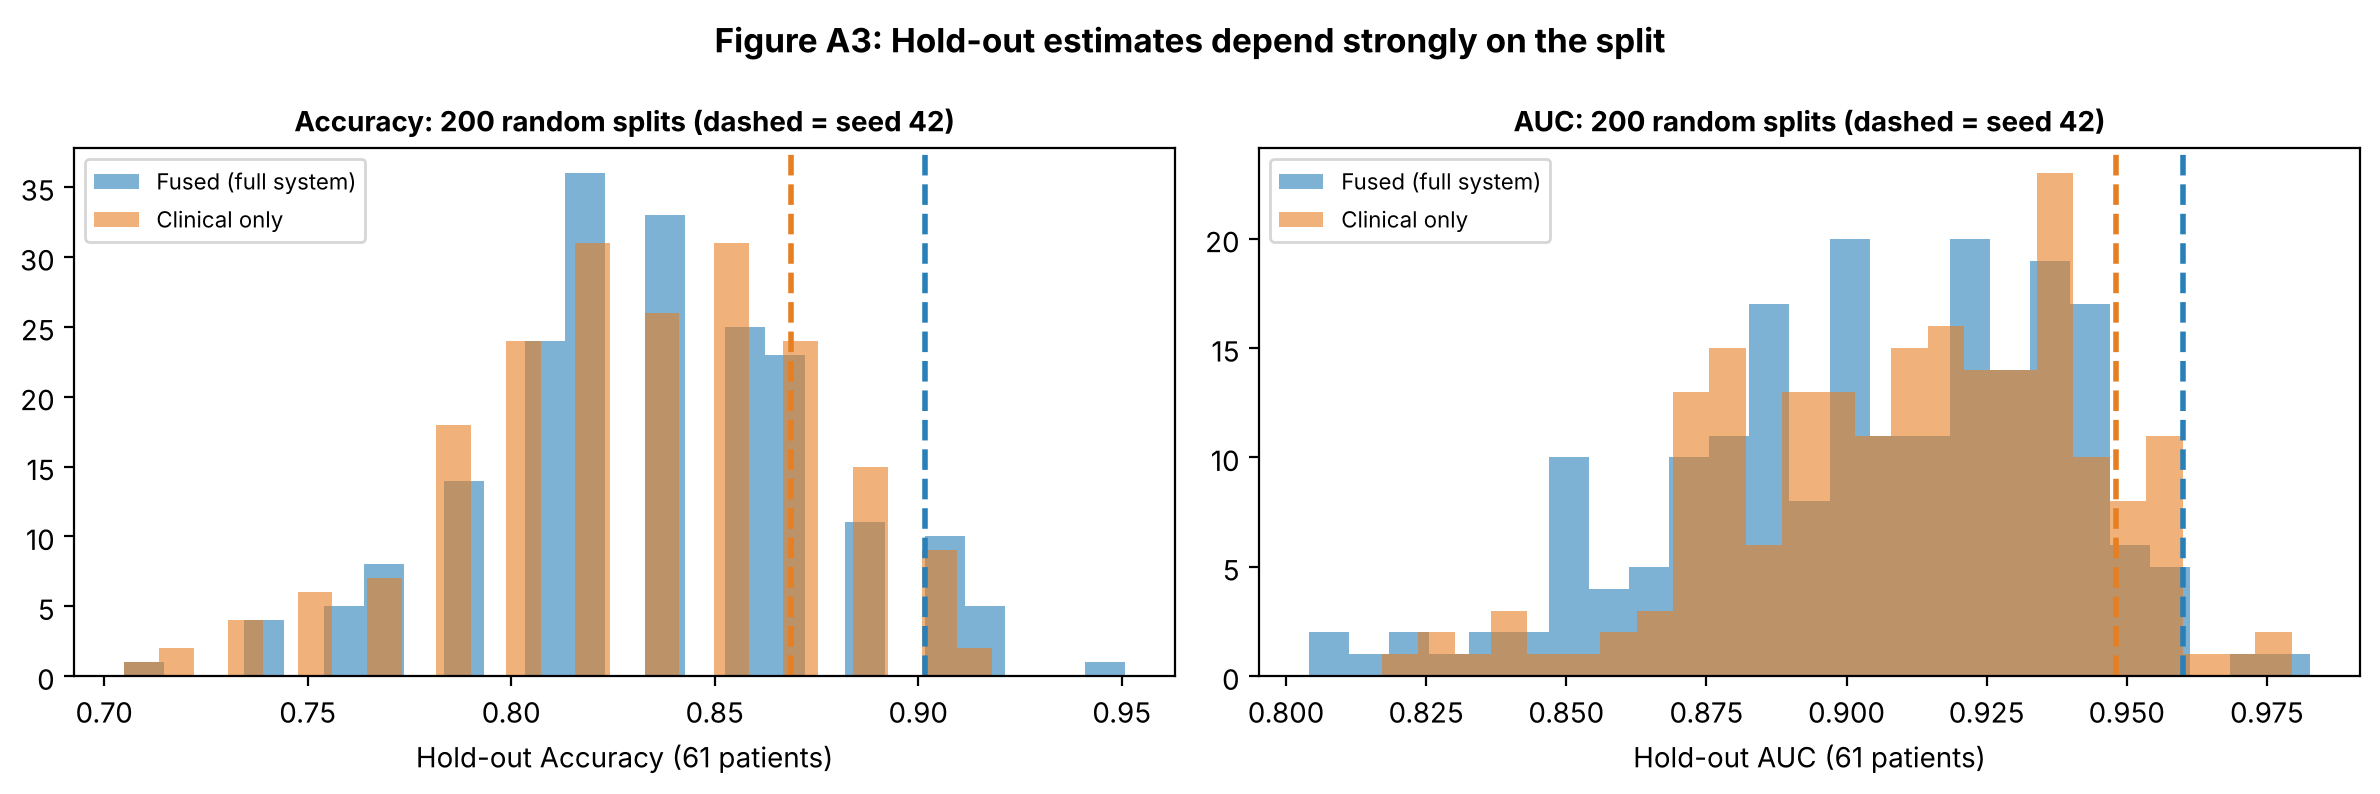
\includegraphics[width=\linewidth]{figA3_holdout_sensitivity.png}
\caption{Distribution of hold-out accuracy and AUC over \hoN{} random 80/20 splits; dashed lines mark the seed-42 split used in v4.}
\label{fig:a3}
\end{figure}

\subsection{Robustness and Edge Cases (RQ3)}
A proxy block could still be useful in harder conditions even if it adds nothing on clean data. Table~\ref{tab:e5} and Fig.~\ref{fig:a4} apply 16 perturbations identically to the fused and clinical-only systems: training label noise (5--20\%), missing values at test time or in both training and test data (10--30\%, MCAR), Gaussian measurement noise (0.25--1~SD), reduced training sets (25--75\%), and clinically motivated missing modalities. Across all scenarios $\Delta$AUC lies between \robMinD{} and \robMaxD{}, and \robNsig{} of \robN{} comparisons are significant after Holm correction. The proxy block does not make the model more robust to label noise (20\% noise: \robNoiseFu{} vs.\ \robNoiseCl{}) or to small training sets (25\%: \robSmallFu{} vs.\ \robSmallCl{}). The most clinically relevant edge case is a patient without angiography or a thallium scan (\texttt{ca}, \texttt{thal} unavailable), where ECG-derived information might be expected to matter most. Even there the fused and clinical systems perform equally (\robNoAngioFu{} vs.\ \robNoAngioCl{}; $\Delta$ \robNoAngioD{}). Removing the exercise test costs little (AUC \robNoExFu{}), whereas resting data alone (no exercise test, no angiography or thallium) drops AUC to \robRestFu{}. This identifies \texttt{ca}, \texttt{thal} and \texttt{cp} as the dominant information sources.

\begin{table*}[!t]
\centering
\scriptsize
\caption{Robustness and edge cases. Each perturbation is applied identically to the fused and the clinical-only system.}
\label{tab:e5}
\setlength{\tabcolsep}{3pt}
\begin{adjustbox}{max width=\linewidth}
\begin{tabular}{lccccc}
\toprule
Scenario (3$\times$10-fold CV) & AUC fused & AUC clin. & $\Delta$AUC [95\% CI] & $p_{\mathrm{Holm}}$ & Sens. fused / clin. \\
\midrule
Baseline (no perturbation) & 0.901 & 0.907 & -0.006 [-0.018, +0.006] & 1.000 & 0.780 / 0.787 \\
Training label noise 5\% & 0.894 & 0.906 & -0.011 [-0.025, +0.002] & 1.000 & 0.779 / 0.789 \\
Training label noise 10\% & 0.889 & 0.901 & -0.012 [-0.029, +0.005] & 1.000 & 0.791 / 0.787 \\
Training label noise 20\% & 0.863 & 0.877 & -0.014 [-0.033, +0.005] & 1.000 & 0.741 / 0.780 \\
Test-time missing values (MCAR) 10\% & 0.892 & 0.894 & -0.002 [-0.016, +0.012] & 1.000 & 0.753 / 0.741 \\
Test-time missing values (MCAR) 20\% & 0.876 & 0.880 & -0.004 [-0.017, +0.009] & 1.000 & 0.688 / 0.671 \\
Test-time missing values (MCAR) 30\% & 0.863 & 0.862 & +0.002 [-0.014, +0.017] & 1.000 & 0.633 / 0.616 \\
Missing values in train AND test 20\% & 0.878 & 0.880 & -0.002 [-0.016, +0.012] & 1.000 & 0.770 / 0.756 \\
Measurement noise $\sigma$=0.25$\times$SD (test) & 0.899 & 0.906 & -0.007 [-0.019, +0.005] & 1.000 & 0.782 / 0.789 \\
Measurement noise $\sigma$=0.5$\times$SD (test) & 0.901 & 0.904 & -0.003 [-0.017, +0.012] & 1.000 & 0.794 / 0.789 \\
Measurement noise $\sigma$=1.0$\times$SD (test) & 0.898 & 0.900 & -0.003 [-0.022, +0.017] & 1.000 & 0.789 / 0.785 \\
Training set reduced to 25\% & 0.872 & 0.882 & -0.010 [-0.029, +0.008] & 1.000 & 0.763 / 0.762 \\
Training set reduced to 50\% & 0.886 & 0.900 & -0.014 [-0.036, +0.008] & 1.000 & 0.777 / 0.794 \\
Training set reduced to 75\% & 0.896 & 0.909 & -0.013 [-0.028, +0.002] & 1.000 & 0.794 / 0.794 \\
No angiography/thallium (ca, thal unavailable) & 0.864 & 0.866 & -0.002 [-0.015, +0.012] & 1.000 & 0.767 / 0.760 \\
No exercise test (thalach, exang, oldpeak, slope) & 0.905 & 0.901 & +0.004 [-0.003, +0.012] & 1.000 & 0.782 / 0.775 \\
Resting data only (both unavailable) & 0.837 & 0.834 & +0.003 [-0.009, +0.015] & 1.000 & 0.784 / 0.770 \\
\bottomrule
\end{tabular}
\end{adjustbox}
\end{table*}


\begin{figure}[!t]
\centering
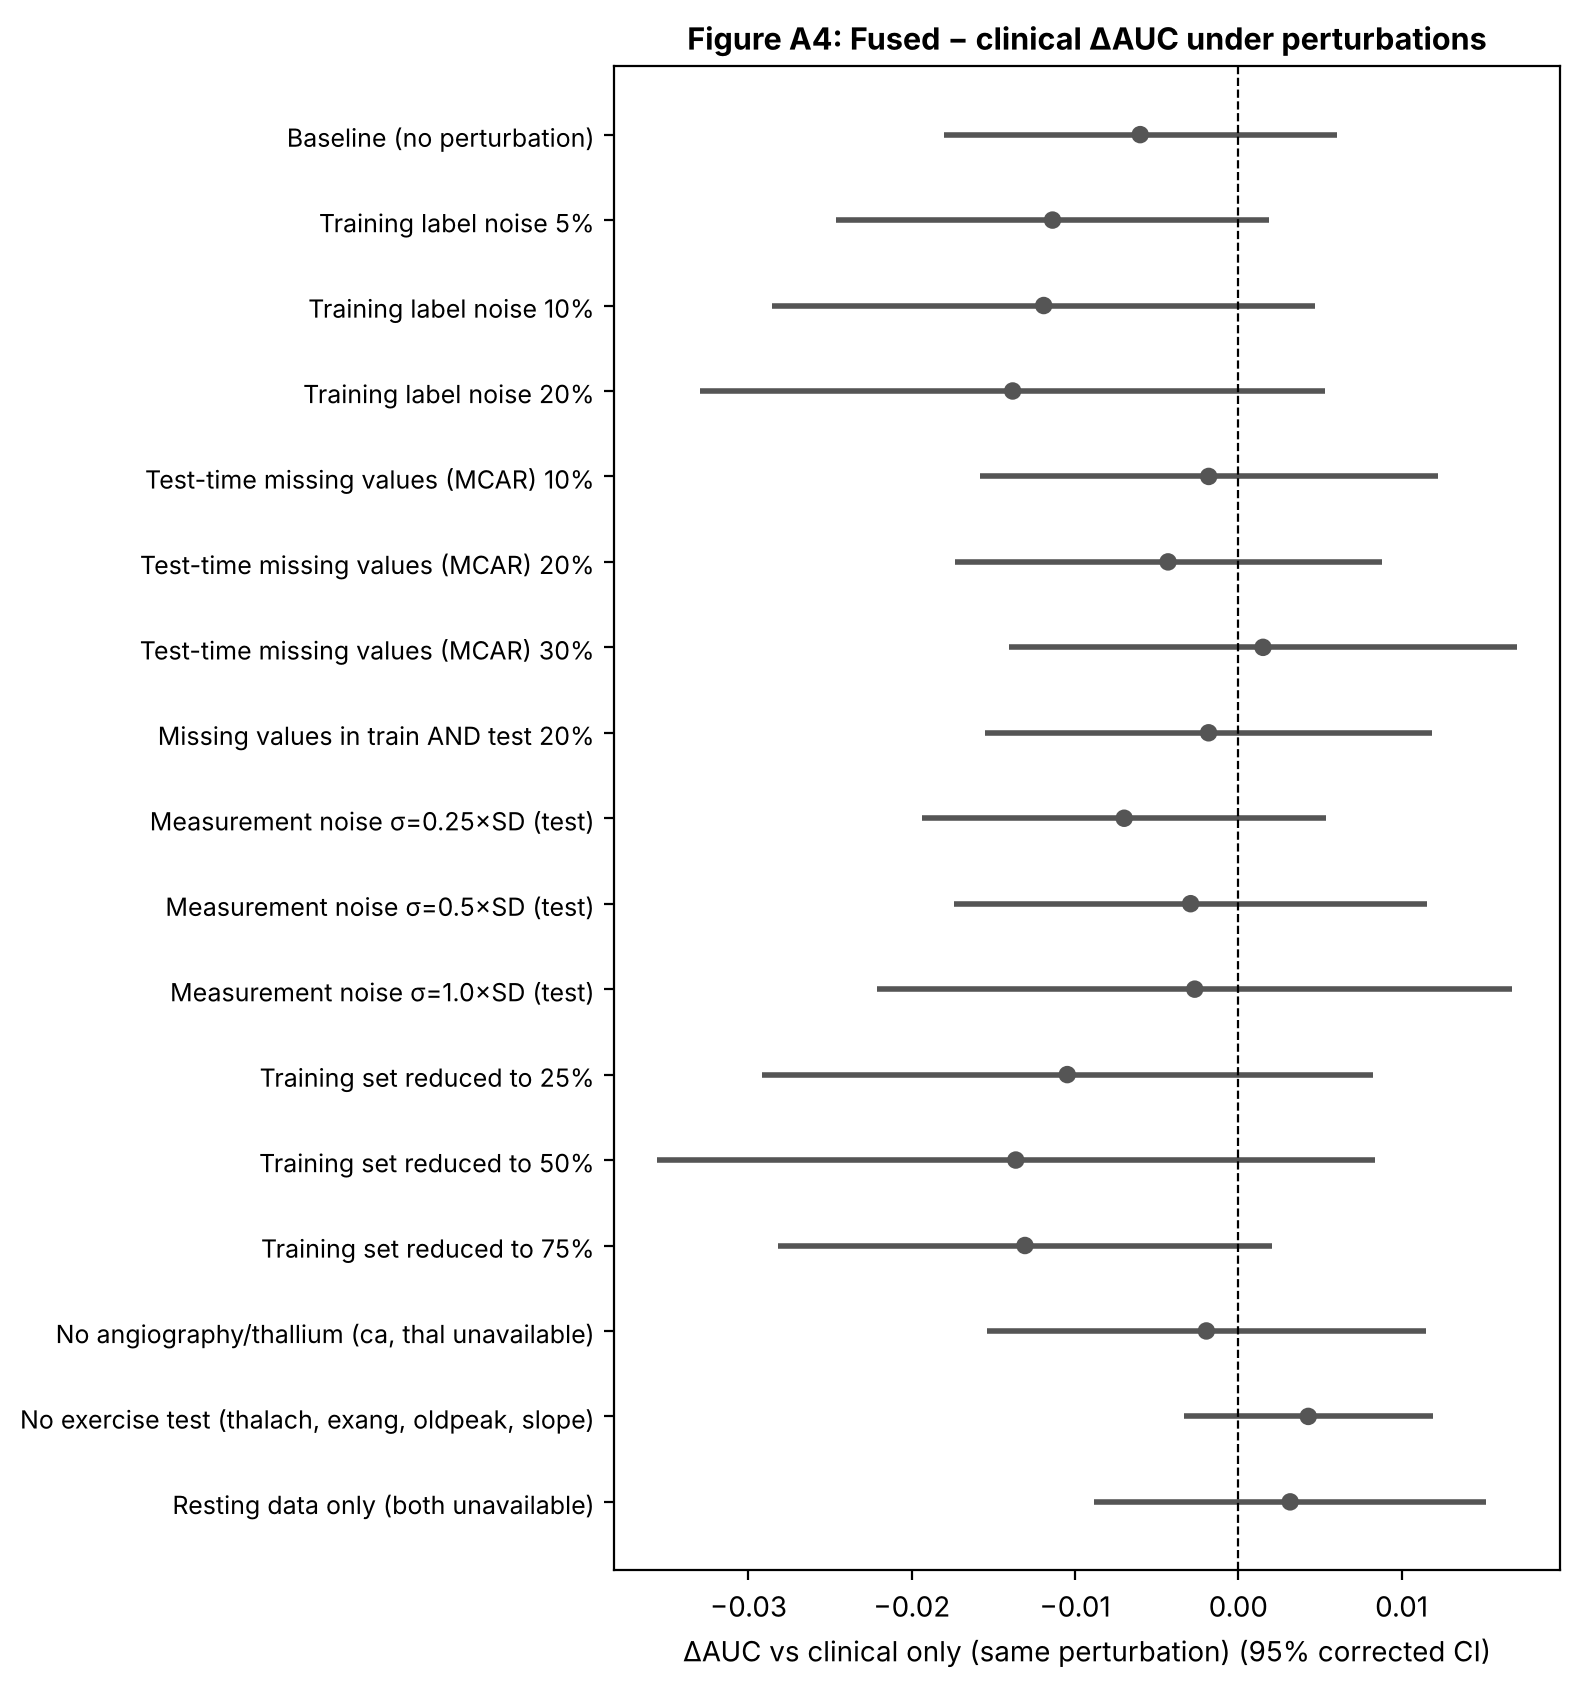
\includegraphics[width=\linewidth]{figA4_robustness.png}
\caption{Fused minus clinical-only $\Delta$AUC under each perturbation (3$\times$10-fold CV, paired).}
\label{fig:a4}
\end{figure}

\textbf{Subgroups.} Table~\ref{tab:subgroups} reports out-of-fold performance by sex, age, chest-pain type and resting ECG. The proxy block does not significantly help any subgroup; every subgroup $\Delta$AUC CI includes zero. Discrimination is similar in women and men but lower in patients aged $\geq$55 years than in younger patients, and lowest in patients with symptomatic chest pain (cp~1--3), where CAD is less prevalent and the dominant predictor \texttt{cp} carries less information. These are the groups in which the model would most need improvement before clinical use.

\begin{table}[!t]
\centering
\scriptsize
\caption{Subgroup performance (out-of-fold predictions averaged over 5 repeats; bootstrap CIs).}
\label{tab:subgroups}
\setlength{\tabcolsep}{3pt}
\begin{adjustbox}{max width=\linewidth}
\begin{tabular}{lccccc}
\toprule
Subgroup & n & Dis. & AUC fused & AUC clin. & $\Delta$AUC [95\% CI] \\
\midrule
All patients & 303 & 139 & 0.900 & 0.905 & -0.005 [-0.014, +0.003] \\
Female & 97 & 25 & 0.899 & 0.908 & -0.008 [-0.026, +0.007] \\
Male & 206 & 114 & 0.883 & 0.884 & -0.002 [-0.013, +0.009] \\
Age < 55 & 143 & 44 & 0.933 & 0.935 & -0.003 [-0.016, +0.013] \\
Age $\geq$ 55 & 160 & 95 & 0.853 & 0.858 & -0.005 [-0.018, +0.010] \\
Asymptomatic chest pain (cp=4) & 144 & 105 & 0.882 & 0.890 & -0.008 [-0.028, +0.008] \\
Symptomatic chest pain (cp=1--3) & 159 & 34 & 0.802 & 0.815 & -0.012 [-0.041, +0.014] \\
Normal resting ECG & 151 & 56 & 0.885 & 0.884 & +0.000 [-0.013, +0.014] \\
Abnormal resting ECG & 152 & 83 & 0.912 & 0.920 & -0.008 [-0.018, +0.001] \\
\bottomrule
\end{tabular}
\end{adjustbox}
\end{table}


\subsection{Ordinal Encoding and Calibration}
One-hot coding of \texttt{cp}, \texttt{restecg}, \texttt{slope} and \texttt{thal} gives AUC \calOnehotAUC{} for the full system (Table~\ref{tab:e6}), no different from ordinal coding, because the dominant tree and RBF members are insensitive to the coding. Calibration matters more for clinical use than a third decimal of AUC~\cite{vancalster2019}. The soft-voting ensemble has a calibration slope of \calFull{}: its probabilities are \emph{under-confident}, compressed towards 0.5 by averaging. The Brier score is \brierFull{}. Platt scaling moves the slope towards 1 (\calPlattSlope{}; Brier \calPlattBrier{}) without changing discrimination. Isotonic regression over-corrects (slope \calIsoSlope{}, i.e.\ over-confident; Brier \calIsoBrier{}), as is typical when a non-parametric calibrator is fitted on about 240 patients (Fig.~\ref{fig:a5}). In this cohort Platt scaling therefore performed better than isotonic regression. Any calibration should be re-estimated in the target population before clinical use. Equal voting weights are adequate: learned weights (stacking) give the same AUC.

\begin{table*}[!t]
\centering
\scriptsize
\caption{Ordinal versus one-hot encoding and probability calibration.}
\label{tab:e6}
\setlength{\tabcolsep}{3pt}
\begin{adjustbox}{max width=\linewidth}
\begin{tabular}{lcccc}
\toprule
Variant & AUC & Brier & Cal.\ slope & $\Delta$AUC [95\% CI] \\
\midrule
Full system (clinical + ECG-proxy, SMOTE, soft voting) & 0.902 & 0.127 & 1.37 & -- \\
One-hot cp/restecg/slope/thal (full system) & 0.903 & 0.127 & 1.39 & +0.002 [-0.007, +0.011] \\
One-hot cp/restecg/slope/thal (clinical only) & 0.907 & 0.126 & 1.35 & +0.006 [-0.009, +0.020] \\
Clinical only & 0.906 & 0.126 & 1.37 & +0.004 [-0.009, +0.017] \\
Platt-calibrated soft voting & 0.900 & 0.125 & 1.13 & -0.001 [-0.006, +0.004] \\
Isotonic-calibrated soft voting & 0.900 & 0.127 & 0.56 & -0.001 [-0.010, +0.008] \\
$-$ SMOTE (no resampling) & 0.900 & 0.128 & 1.41 & -0.002 [-0.009, +0.006] \\
\bottomrule
\end{tabular}
\end{adjustbox}
\end{table*}


\begin{figure}[!t]
\centering
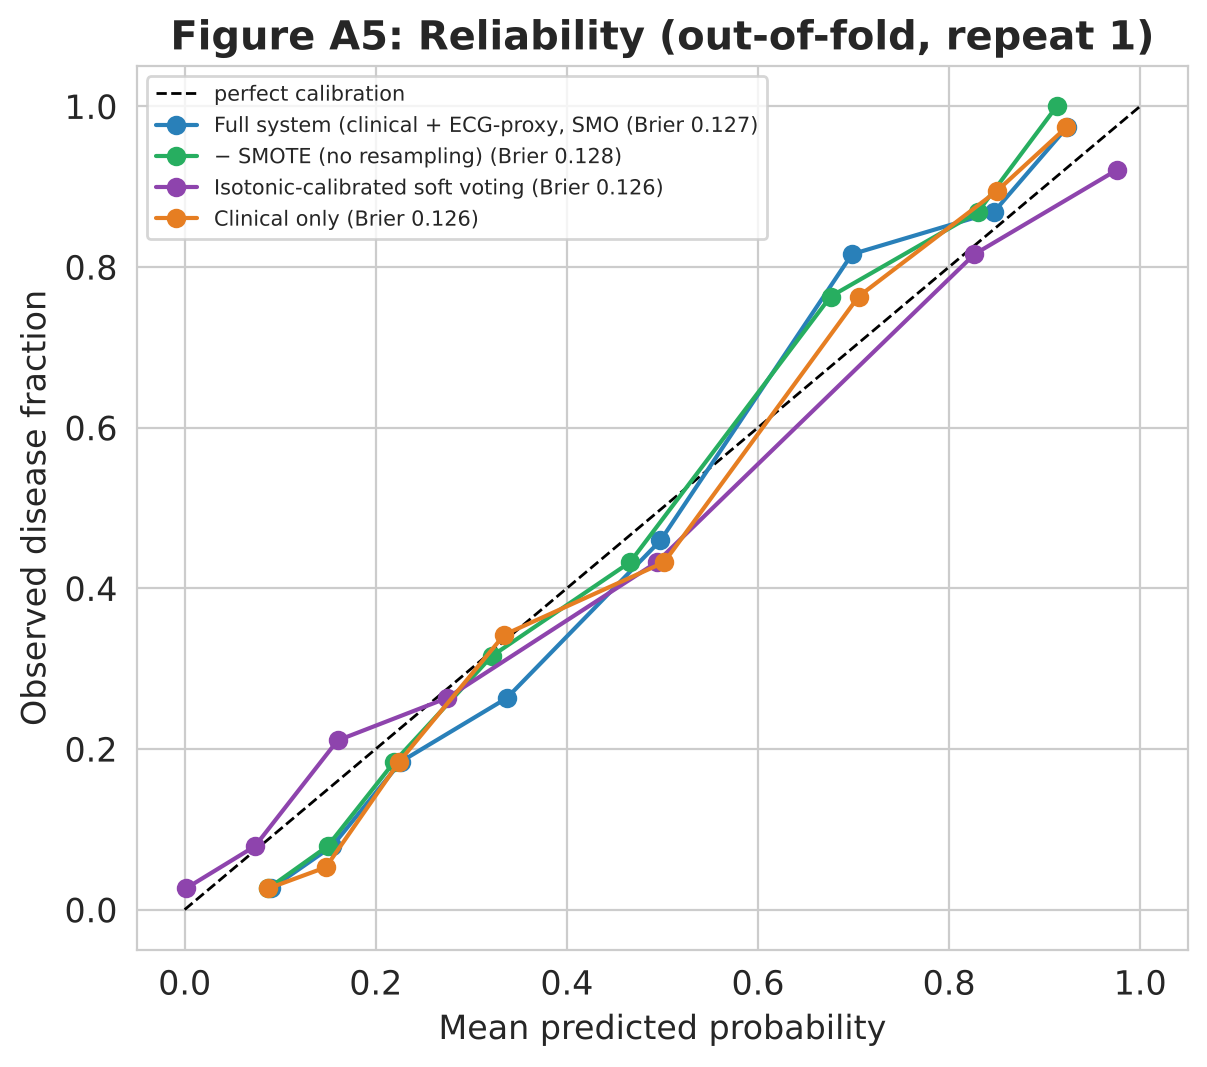
\includegraphics[width=0.85\linewidth]{figA5_calibration.png}
\caption{Reliability diagram of out-of-fold probabilities (repeat 1).}
\label{fig:a5}
\end{figure}

\subsection{External Validation on Three Further Hospitals (RQ3)}
All earlier results are internal to Cleveland. Table~\ref{tab:sites} shows that the three other UCI sites differ markedly from it. CAD prevalence ranges from 36\% (Hungary) to 94\% (Switzerland), and the two strongest Cleveland predictors are mostly unavailable: \texttt{ca} is missing for 96--99\% and \texttt{thal} for 42--90\% of patients. Models trained on all 303 Cleveland patients and applied unchanged (Table~\ref{tab:e7}, Fig.~\ref{fig:a6}) reach AUC \extHunFu{} in Hungary, \extSwiFu{} in Switzerland and \extVaFu{} at VA Long Beach (clinical-only: \extHunCl{}, \extSwiCl{}, \extVaCl{}). Fused and clinical-only models do not differ at any site (fused$-$clinical $\Delta$AUC with bootstrap CI: \extDeltaList{}).

A second edge case emerges here. When \texttt{ca} and \texttt{thal} are missing, median imputation fills them with Cleveland's medians (0 vessels, normal thallium), the values most typical of \emph{healthy} patients. Sensitivity therefore collapses at the external sites (Table~\ref{tab:e7}). Training without \texttt{ca}, \texttt{thal} and \texttt{slope} restores sensitivity to 0.77--0.85 and improves calibration (lower Brier) at the cost of specificity, and at VA it also improves AUC. A model should therefore be trained on the features that will actually be available at deployment rather than relying on imputation of its most important inputs. Cholesterol is recorded as 0~mg/dL for all 123 Swiss and 49 VA patients. Treating these values as missing rather than literally changes external AUC by at most 0.004, because cholesterol carries little weight in the model (\texttt{E7\_chol\_zero\_edge\_case.csv} in the repository).

\begin{table}[!t]
\centering
\scriptsize
\caption{Characteristics of the four UCI heart-disease sites (chol = 0 treated as missing).}
\label{tab:sites}
\setlength{\tabcolsep}{3pt}
\begin{adjustbox}{max width=\linewidth}
\begin{tabular}{lcccccc}
\toprule
Site & n & Prev. & ca miss. & thal miss. & slope miss. & chol miss. \\
\midrule
Cleveland & 303 & 45.9\% & 1\% & 1\% & 0\% & 0\% \\
Hungary & 294 & 36.1\% & 99\% & 90\% & 65\% & 8\% \\
Switzerland & 123 & 93.5\% & 96\% & 42\% & 14\% & 100\% \\
VA Long Beach & 200 & 74.5\% & 99\% & 83\% & 51\% & 28\% \\
\bottomrule
\end{tabular}
\end{adjustbox}
\end{table}

\begin{table*}[!t]
\centering
\scriptsize
\caption{External validation: trained on all 303 Cleveland patients, tested unchanged on three other hospitals.}
\label{tab:e7}
\setlength{\tabcolsep}{3pt}
\begin{adjustbox}{max width=\linewidth}
\begin{tabular}{llcccc}
\toprule
Site & Model (trained on Cleveland) & AUC [95\% CI] & Sens. & Spec. & Brier \\
\midrule
Hungary & Clinical only & 0.886 [0.844, 0.927] & 0.557 & 0.963 & 0.143 \\
Hungary & Clinical, without ca/thal/slope & 0.885 [0.844, 0.925] & 0.774 & 0.830 & 0.135 \\
Hungary & Fused (full system) & 0.889 [0.847, 0.931] & 0.670 & 0.931 & 0.133 \\
Hungary & Fused, without ca/thal/slope & 0.883 [0.841, 0.925] & 0.774 & 0.846 & 0.136 \\
Switzerland & Clinical only & 0.785 [0.596, 0.946] & 0.548 & 0.875 & 0.262 \\
Switzerland & Clinical, without ca/thal/slope & 0.792 [0.615, 0.951] & 0.817 & 0.625 & 0.150 \\
Switzerland & Fused (full system) & 0.772 [0.552, 0.959] & 0.574 & 0.750 & 0.250 \\
Switzerland & Fused, without ca/thal/slope & 0.771 [0.560, 0.941] & 0.800 & 0.625 & 0.154 \\
VA Long Beach & Clinical only & 0.721 [0.635, 0.803] & 0.463 & 0.784 & 0.261 \\
VA Long Beach & Clinical, without ca/thal/slope & 0.751 [0.672, 0.828] & 0.846 & 0.451 & 0.168 \\
VA Long Beach & Fused (full system) & 0.709 [0.622, 0.790] & 0.510 & 0.784 & 0.255 \\
VA Long Beach & Fused, without ca/thal/slope & 0.754 [0.674, 0.826] & 0.839 & 0.490 & 0.176 \\
\bottomrule
\end{tabular}
\end{adjustbox}
\end{table*}


\begin{figure}[!t]
\centering
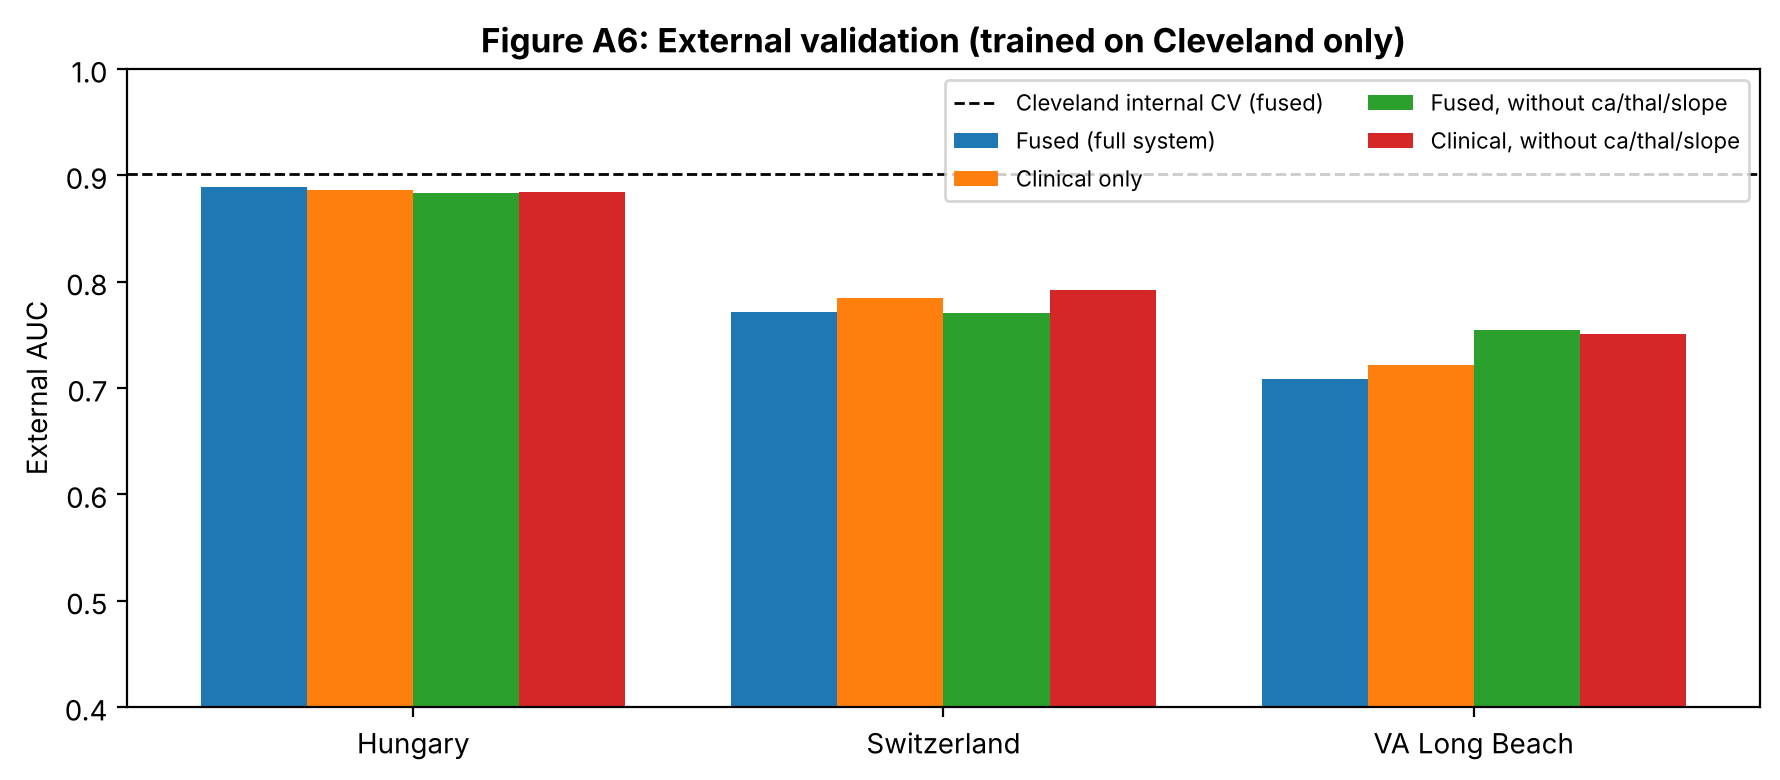
\includegraphics[width=\linewidth]{figA6_external.png}
\caption{External AUC of models trained on Cleveland only (dashed: Cleveland internal CV).}
\label{fig:a6}
\end{figure}

\subsection{SHAP Stability (RQ4)}
Attribution stability across 50 folds and 10 seeds, and agreement with permutation importance, are reported with the interpretation results in Section~VII (Tables~\ref{tab:e8} and~\ref{tab:shaptop}).

\subsection{Cross-Attention in the Dual-Branch Network}
Table~\ref{tab:e9} compares six networks trained with identical preprocessing, SMOTE and training budget. The numerical check confirms the derivation of Section~IV-C: with sequence length 1 every attention weight equals 1.000000, and replacing the ECG query with random values leaves the output unchanged. Consistent with this, the v4 architecture (AUC \xattnAUC{}) performs like its linear equivalent (\linearAUC{}) and like plain concatenation (\concatAUC{}; $\Delta$ \dConcat{}). A token-level variant, in which each ECG-proxy feature attends over the 13 clinical features so that attention can actually weight them, reaches \tokensAUC{} ($\Delta$ \dTokens{}). The token-level variant only reaches the level of the clinical-only MLP (\mlpClinAUC{}); no network exceeds it, and all remain below the soft-voting ensemble (\fullAUC{}). Adding the proxy block to an MLP actually lowers AUC (single MLP on all 36 features), as expected when 303 patients are spread over more inputs. We therefore remove cross-attention from the proposed system and report the dual-branch network only as an ablation.

\begin{table*}[!t]
\centering
\scriptsize
\caption{Dual-branch networks with and without cross-attention (identical preprocessing, SMOTE and training budget).}
\label{tab:e9}
\setlength{\tabcolsep}{3pt}
\begin{adjustbox}{max width=\linewidth}
\begin{tabular}{lcccc}
\toprule
Model (3$\times$10-fold CV) & AUC [95\% CI] & Acc. & Sens. & $\Delta$AUC vs L=1 attention \\
\midrule
Full system (clinical + ECG-proxy, SMOTE, soft voting) & 0.901 [0.859, 0.944] & 0.824 & 0.780 & +0.015 [-0.018, +0.047] \\
$-$ ECG-proxy block (clinical only) & 0.907 [0.865, 0.950] & 0.827 & 0.787 & +0.021 [-0.013, +0.054] \\
DL: clinical-only MLP (Section 14) & 0.892 [0.848, 0.936] & 0.821 & 0.787 & +0.006 [-0.023, +0.035] \\
DL: single MLP on all 36 features & 0.866 [0.826, 0.906] & 0.793 & 0.763 & -0.021 [-0.052, +0.010] \\
DL: dual branch + concatenation & 0.878 [0.828, 0.927] & 0.813 & 0.765 & -0.009 [-0.030, +0.012] \\
DL: dual branch + cross-attention (L=1, paper) & 0.887 [0.840, 0.933] & 0.812 & 0.791 & -- \\
DL: dual branch + linear layer ($\equiv$ L=1 attention) & 0.885 [0.843, 0.927] & 0.814 & 0.767 & -0.002 [-0.023, +0.019] \\
DL: dual branch + token-level cross-attention & 0.893 [0.852, 0.934] & 0.815 & 0.813 & +0.006 [-0.023, +0.036] \\
\bottomrule
\end{tabular}
\end{adjustbox}
\end{table*}


\subsection{PTB-XL ECG Branch}
The parallel ECG benchmark (D2; PTB-XL normal versus abnormal) was ablated in the same way (Table~\ref{tab:e10}). Lead~II with Efficient tsfresh features reaches AUC \ecgRefAUC{}. The choice of lead matters: V5 performs as well as Lead~II (\ecgVFiveAUC{}), while Lead~I (\ecgLeadIAUC{}) and V1 (\ecgVOneAUC{}) are weaker. The rich feature set is essential: the 10 Minimal statistics of Lead~II reach only \ecgMinIIAUC{} (significant drop), and 10 Minimal statistics from each of the 12 leads reach \ecgTwelveMinAUC{}. Adding the 12-lead statistics to the Lead-II descriptors gives \ecgTwelvePlusAUC{}, a small, non-significant gain, so with handcrafted statistics and $N=303$ most of the accessible information is already in one well-chosen lead. Fitting VarianceThreshold and scaling on all records, as in v4, has no measurable effect, and neither SMOTE nor the random forest of v4 improves on the reference. Increasing the training set to 1{,}212 records does not raise AUC appreciably (Table~\ref{tab:e10size}; \ecgSizeList{}), although accuracy and the precision of the estimate improve. Substantial gains from raw ECGs are known to require learned representations and far larger datasets~\cite{ribeiro2020}. Signal quality matters: records with PTB-XL noise or electrode annotations ($n=\ecgNoisyN{}$) are classified with AUC \ecgNoisyAUC{} versus \ecgCleanAUC{} for clean records.

\begin{table*}[!t]
\centering
\scriptsize
\caption{PTB-XL ECG-branch (D2) ablation, 303 records, 5$\times$10-fold CV.}
\label{tab:e10}
\setlength{\tabcolsep}{3pt}
\begin{adjustbox}{max width=\linewidth}
\begin{tabular}{lcccc}
\toprule
ECG-branch variant (PTB-XL labels) & AUC [95\% CI] & Acc. & $\Delta$AUC [95\% CI] & $p_{\mathrm{Holm}}$ \\
\midrule
Lead II, Efficient tsfresh, soft voting (reference) & 0.819 [0.766, 0.871] & 0.725 & -- & -- \\
VarianceThreshold + scaling fitted on all records & 0.820 [0.766, 0.874] & 0.727 & +0.001 [-0.007, +0.009] & 1.000 \\
Random Forest only (Section 13 best) & 0.786 [0.732, 0.839] & 0.695 & -0.033 [-0.073, +0.007] & 0.656 \\
No SMOTE & 0.807 [0.752, 0.862] & 0.717 & -0.012 [-0.040, +0.017] & 1.000 \\
Minimal tsfresh (10 features), Lead II & 0.666 [0.593, 0.739] & 0.589 & -0.153 [-0.234, -0.072] & 0.004 \\
Lead I, Efficient & 0.724 [0.659, 0.789] & 0.656 & -0.095 [-0.176, -0.014] & 0.182 \\
Lead V1, Efficient & 0.752 [0.695, 0.810] & 0.684 & -0.067 [-0.145, +0.012] & 0.656 \\
Lead V5, Efficient & 0.819 [0.762, 0.876] & 0.743 & -0.000 [-0.062, +0.061] & 1.000 \\
12-lead Minimal tsfresh (120 features) & 0.768 [0.714, 0.823] & 0.700 & -0.051 [-0.118, +0.016] & 0.680 \\
12-lead Minimal + Lead II Efficient & 0.823 [0.772, 0.874] & 0.740 & +0.004 [-0.024, +0.032] & 1.000 \\
\bottomrule
\end{tabular}
\end{adjustbox}
\end{table*}

\begin{table}[!t]
\centering
\scriptsize
\caption{PTB-XL Lead-II branch: effect of the number of training records (3$\times$10-fold CV).}
\label{tab:e10size}
\setlength{\tabcolsep}{3pt}
\begin{adjustbox}{max width=\linewidth}
\begin{tabular}{cccc}
\toprule
Records & Patients & AUC [95\% CI] & Accuracy [95\% CI] \\
\midrule
303 & 302 & 0.823 [0.766, 0.880] & 0.721 [0.665, 0.778] \\
606 & 605 & 0.800 [0.760, 0.841] & 0.727 [0.686, 0.768] \\
1212 & 1200 & 0.825 [0.801, 0.848] & 0.757 [0.730, 0.784] \\
\bottomrule
\end{tabular}
\end{adjustbox}
\end{table}


\begin{figure}[!t]
\centering
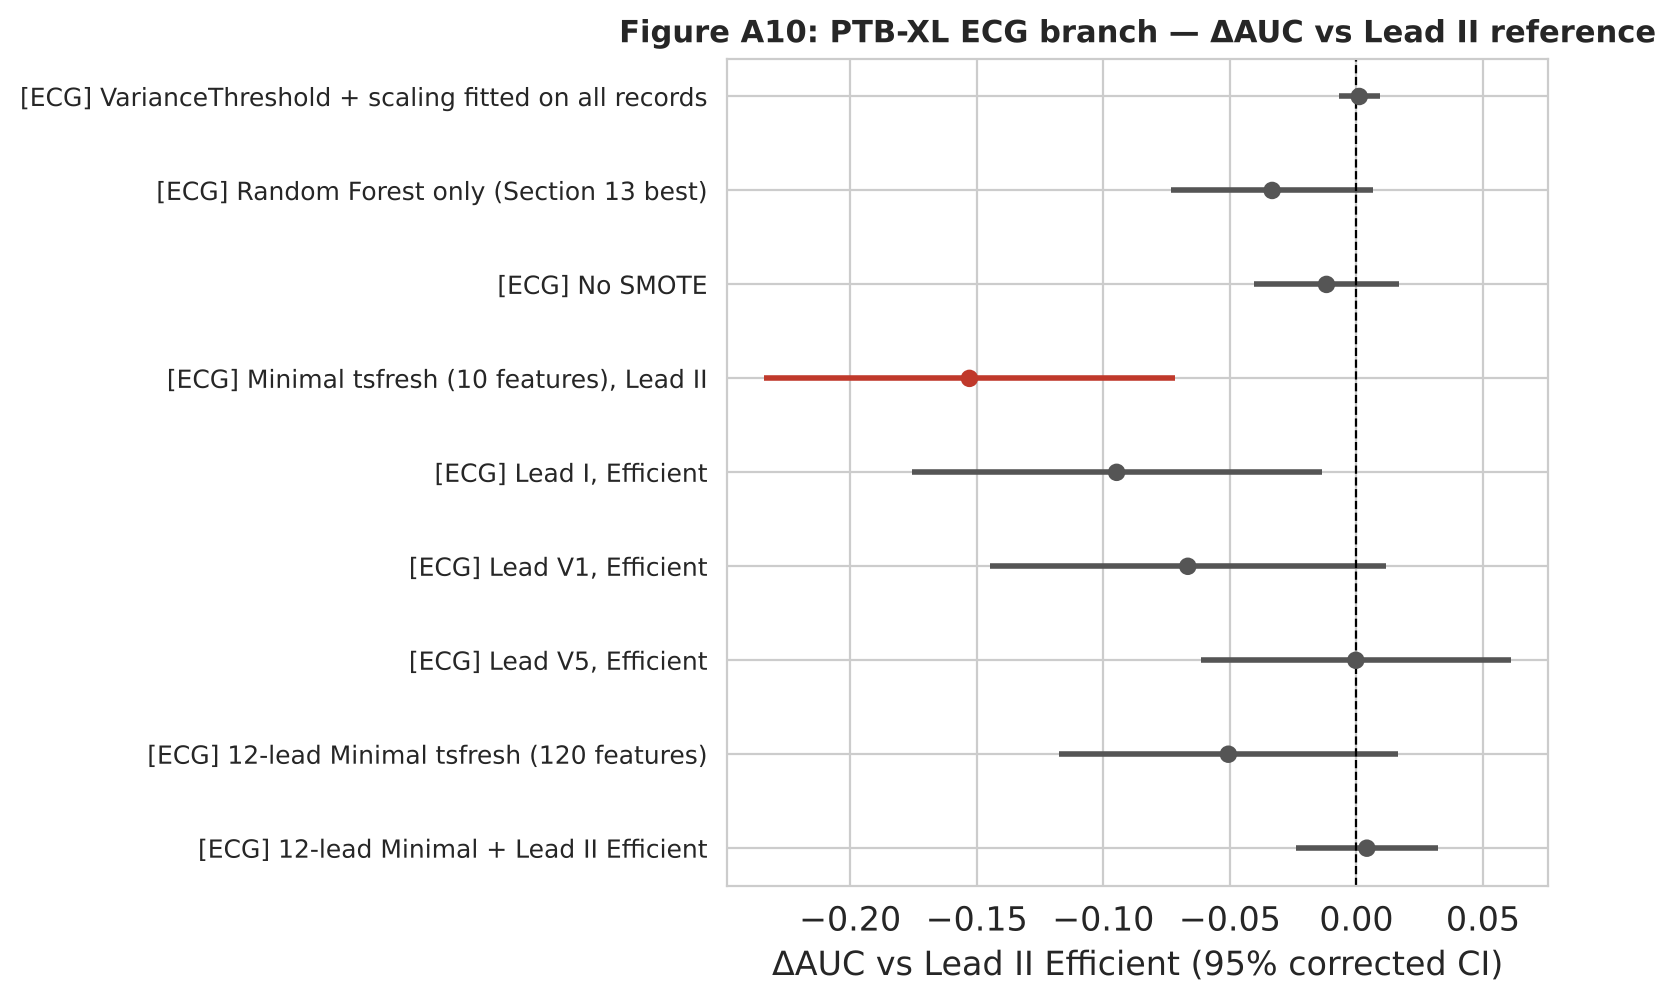
\includegraphics[width=\linewidth]{figA10_ptbxl_branch.png}
\caption{PTB-XL ECG-branch ablation: $\Delta$AUC versus Lead~II with Efficient tsfresh features.}
\label{fig:a10}
\end{figure}

\subsection{Summary: Which Claims Survive?}
Table~\ref{tab:verdict} re-tests each quantitative claim of the v4 manuscript.

\begin{table*}[!t]
\centering
\scriptsize
\caption{Claims of the v4 manuscript re-tested under the controlled protocol. A claim is supported only if the 95\% CI of the paired difference excludes zero in the claimed direction.}
\label{tab:verdict}
\setlength{\tabcolsep}{3pt}
\begin{adjustbox}{max width=\linewidth}
\begin{tabular}{p{4.6cm}p{2.6cm}p{5.6cm}p{3.6cm}}
\toprule
Claim in the v4 manuscript & v4 value & Controlled estimate [95\% CI] & Verdict \\
\midrule
ECG-proxy fusion improves accuracy over clinical-only & +7.04 pp & -0.262 pp [-2.683, +2.158] & Not supported (CI includes 0) \\
ECG-proxy fusion improves AUC over clinical-only & +0.87 pp (0.9535 vs 0.9459) & -0.004 [-0.017, +0.009] & Not supported (CI includes 0) \\
Removing the ECG-proxy layer lowers AUC & $\approx$ $-$0.06 & +0.004 [-0.009, +0.017] & Not supported (CI includes 0) \\
Removing SMOTE causes the largest drop & $\approx$ $-$3.3\% accuracy & +1.058 pp [-0.584, +2.700] & Not supported (CI includes 0) \\
Removing SMOTE lowers AUC & "noticeable drop" & -0.002 [-0.009, +0.006] & Not supported (CI includes 0) \\
Ensemble beats a single (XGBoost) classifier & AUC $-$0.014 without ensemble & -0.007 [-0.020, +0.006] & Not supported (CI includes 0) \\
Feature engineering contributes & AUC $-$0.005 without it & -0.003 [-0.023, +0.018] & Not supported (CI includes 0) \\
ECG-proxy block beats an equal-size non-ECG block & (implied) & -0.002 [-0.020, +0.016] & Not supported (CI includes 0) \\
Cross-attention improves the dual-branch network & (implied by MCF-BiModNet) & +0.009 [-0.012, +0.030] & Not supported (CI includes 0) \\
SHAP ranking is a stable basis for clinical interpretation & thal, ca, cp, oldpeak dominate & fold-to-fold Spearman $\rho$ = 0.90; top-5 Jaccard = 0.74 & Partly supported (top features stable, tail unstable) \\
Performance generalises beyond Cleveland & (not tested) & Hungary AUC=0.889, Switzerland AUC=0.772, VA Long Beach AUC=0.709 & Lower AUC at all external sites; fused $\approx$ clinical \\
Hold-out accuracy 88.52\% is representative & 0.8852 (seed 42) & 0.833 over 200 splits (seed 42 = 95th pct) & Optimistic single split \\
\bottomrule
\end{tabular}
\end{adjustbox}
\end{table*}



